\graphicspath{{chapters/chapter4/}}
\chapter{Methods} \label{chapter3}

This section summarizes the theory behind the techniques implemented in the experiments.  The first paragraph concerns Logistic Regression, a classic supervised machine learning method for classification. Then follows a section with a brief description of the implemented deep learning architectures.  Finally, the general framework of CBM is presented.
\section{Logistic Regression}
\textbf{Logistic Regression(LR)} is a supervised learning classification algorithm used to predict the probability of an input to belong to a target class. The nature of target or dependent variable is dichotomous, which means that the probability of the output to belong to a class will be $P$, while $(1-P)$ if it belongs to the other class(where $P$ is a number between 0 and 1).\\ 
Logistic Regression is achieved by applying Sigmoid function on linear regression:
\begin{equation}
p = \frac{1}{1 + e^{-(\beta_0 + \beta_1 x_1 + \beta_2 x_2 + ... +\beta_n x_n)}    }
\label{LReq}
\end{equation}
The Linear Regression Function is defined as:
\begin{equation}
y = \beta_0 + \beta_1 x_1 + \beta_2 x_2 + ... +\beta_n x_n
\end{equation}
where, $y$ is dependent variable and $x_1, x_2 ...$ and $x_n$ are explanatory input variables, the Sigmoid Function is defined as: 
\begin{equation}
p = \frac{1}{1+e^{-y}}
\end{equation}
The sigmoid Function gives an ‘S’ shaped curve that can take any real-valued number and map it into a value between 0 and 1.
\section{Deep learning architectures}
In the literature, models that perform well in image classification tasks and give good results also in the medical field have been proposed. Complex architectures already pre-trained on large dataset, have been made available in many frameworks, such as Tensorflow\cite{tensorflow2015-whitepaper}.
The following paragraphs describe the structures of the 2 networks used in the experiments, InceptionV3 and ResNet101v2, by using transfer learning.
\subsection{InceptionNet}
\begin{figure}[b]
    \centering
    \begin{subfigure}[b]{0.48\linewidth}        %% or \columnwidth
        \centering
        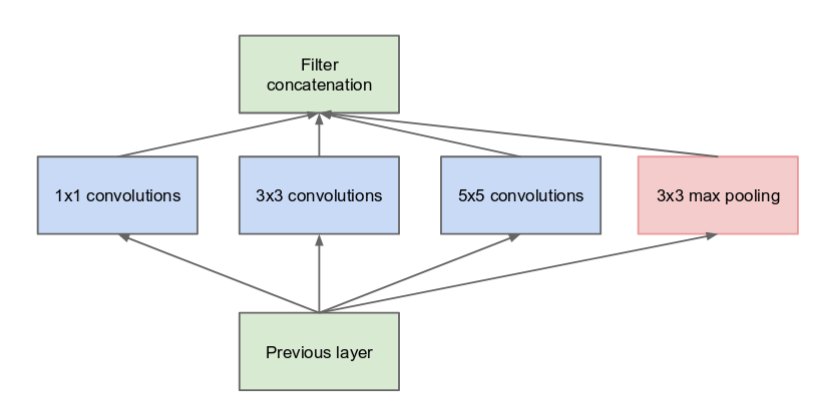
\includegraphics[width=\linewidth]{images/incNet/incnaivemodule.png}
        \caption{Inception Module, naive version}
        \label{fig:incNaiveMod}
    \end{subfigure}
    \begin{subfigure}[b]{0.48\linewidth}        %% or \columnwidth
        \centering
        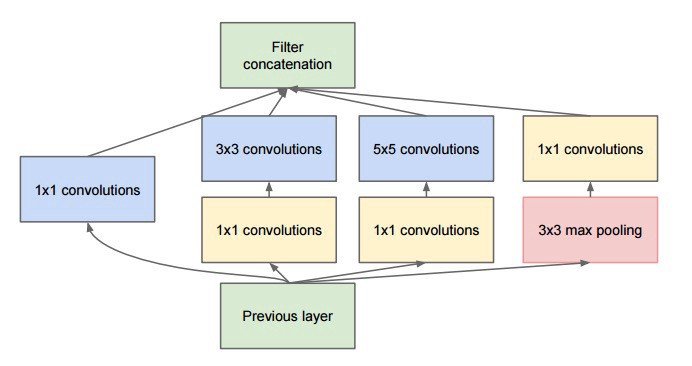
\includegraphics[width=\linewidth]{images/incNet/incmodule.jpeg}
        
        \caption{Inception Module with dimension reductions}
        \label{fig:incModule}
    \end{subfigure}
    \caption{Inception Module}

    \label{fig:NEV_images}
\end{figure}

\begin{figure}[ht]
    \centering
        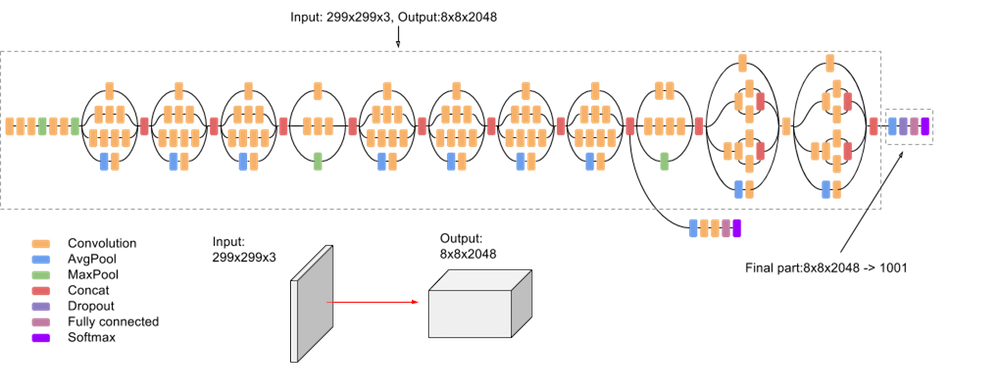
\includegraphics[width=\linewidth]{images/inception_v3_architecture.png}
    \caption{InceptionV3 architecture}
    \label{fig:IncV3}
\end{figure}
\textbf{InceptionV3(IncNet)} is a widely-used image recognition model that has been shown to attain greater than 78.1\% accuracy on the ImageNet dataset~\cite{ImageNet}. The model is the result of many works developed by multiple researchers over the years \cite{IncNet}.\\\\
Inception nets are characterized by a reduced depth at the expense of width; this property allows to have a lower computational complexity than deep networks. \\
This kind of networks are made up of modules called \textbf{Inception Modules}, which allow to have filters with multiple sizes on the same level. The figure~\ref{fig:incNaiveMod} shows the "naive" inception module: it performs convolution on an input with 3 different filters (1x1, 3x3, 5x5). Additionally, max pooling is performed. The outputs are concatenated and sent to the next layer.
Due to the computational effort, extra 1x1 convolutions have been added to these modules, figure~\ref{fig:incModule}.\\
Furthermore, smart factorization methods have been implemented, to factor bigger convolutions(7x7, 5x5) into more convolutions of reduced sizes; they factor the convolutions of the nxn filter size into a combination of 1xn and nx1 convolutions.\\
Other important properties of the network are:
\begin{enumerate}
    \item RMSProp Optimizer.
\item Factorized 7x7 convolutions.
\item BatchNorm in the Auxillary Classifiers.
\item Label Smoothing (A type of regularizing component added to the loss formula that prevents over fitting).
\end{enumerate}
The IncNet is formed by the Inception Modules, and auxiliary classifiers are added in the middle part of the network to apply softmax on the output and to compute an auxiliary loss.\\
The architecture for the InceptionV3 is showed in figure~\ref{fig:IncV3}; the model itself is made up of symmetric and asymmetric building blocks, including convolutions, average pooling, max pooling, concats, dropouts, and fully connected layers. Batchnorm is used extensively throughout the model and applied to activation inputs.
This architecture was trained using a dataset of 1,000 classes from the original ImageNet dataset which was trained with over 1 million training images, while the Tensorflow implementation has 1,001 classes which is due to an additional "background" class not used in the original ImageNet.

\subsection{ResNet}
\textbf{ResNet101V2(ResNet)} is a convolutional neural network that is 101 layers deep. ResNet101V2, as IncNet, was trained on ImageNet.\\
The ResNet architecture is built to address the vanishing gradient problem.
The vanishing gradient problem, argued and discussed in \cite{vanishinGradient}, is a phenomenon that creates difficulties in the training of deep neural networks through the back-propagation of the error through stochastic descent of the gradient. \\
So with ResNet, the gradients can flow directly through the skip connections backwards from later layers to initial filters, solving problem related to back-propagation; this is achieved by introducing a new neural network layer, the Residual Block, shown in figure~\ref{fig:ResBlock}. \\
\begin{figure}[]
    \centering
        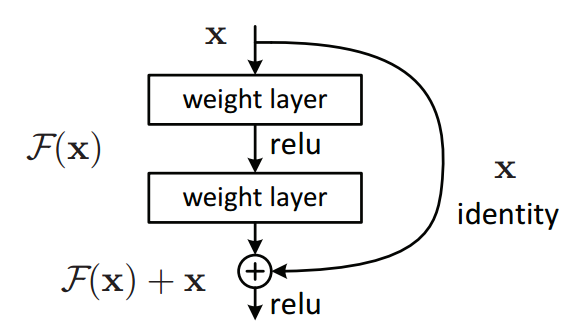
\includegraphics[width=0.7\linewidth]{images/resnet/residualblock.png}
    \caption{Residual Block}
    \label{fig:ResBlock}
\end{figure}
A ResNet is a very deep CNN, consisting of many layers, which with the aid of the technique of skip connection has opened the way to residual networks. Skip connection is the key to training a large number of levels, without losing performance.
Skip connection allows a fast compute of the cost function, by skipping to each residual block during the gradient backpropagation\cite{Resnet}.
\subsection{Transfer Learning}
\textbf{Transfer Learning:}
CNNs can either be trained from scratch where all its parameters are tuned for the problem, or they can be tuned towards the problem from an already pre-trained CNN. This method can be particularly useful for medical applications since it does not require as much training data, which can be hard to get in medical situations \cite{TransferLearningMedicalBackground}. 
A common way to use transfer learning is by loading a model(e.g. ResNet101, InceptionV3) with weights pre-trained on a large database of images annotated with labels (e.g. ImageNet\cite{ImageNet}) and by excluding the fully-connected layer at the top of the network. Generally a new classification layer is added, that is specific to the new task. The model weights are then fine-tuned on the task-specific dataset. In this way, the model should retain basic filters already learned by training on the previous data, resulting in better accuracy and quicker convergence.
\\
\section{Concept BottleNeck Models} \label{sectionCBM}
\textbf{Concept Bottleneck Models(CBM):} are models that first predict an intermediate set of human-specified concepts $c$, then use $c$ to predict the final output $y$\cite{CBM}.
Consider predicting a target $y\in\R$ from input $x\in\R^d$; Firstly, a CBM will predict a vector of $k$ concepts $c\in\R^k$. Then it will use the predicted concepts to estimate the target variable $y$\\
A CBM has the following form, $g(f(x))$, where $f:\R^d \longrightarrow \R^k$ maps an input $x$ into the concepts space and $g:\R^k \longrightarrow \R$ maps concepts into a final prediction. So a CBM will predict $\hat{y}=g(f(x))$ by predicting the concepts $\hat{c}=f(x)$ and $y=g(\hat{c})$. \\
Different ways to learn a concept bottleneck model were studied in \cite{CBM}, but this work only consider:
\begin{enumerate}
    \item The independent bottleneck, that learns ${g}$ and ${f}$ independently: $f$ is trained on the raw inputs and $g$ on the true concepts. But, at test time, ${g}$ takes the predicted concepts $\hat{c}={f}(x)$ 
    \item The sequential bottleneck, first learns ${f}$ in the same way as above. It then uses the concept predictions $\hat{c}$ to learn ${g}$.
\end{enumerate}

\section{Categorical Cross-Entropy Objective function}
\textbf{Categorical Cross-Entropy Loss:} is a Softmax activation plus a Cross-Entropy loss. By using this loss,a CNN will be train a CNN to predict a probability over the 
C classes for each image. It is used for multi-class classification.\\
Softmax function(\ref{softmax}) extends the idea of Sigmoid Function into a multi-class problem,by assigning decimal probabilities to each class. Below softmax function:
\begin{equation}
    softmax(x)_i = \frac{\exp(x_i)}{\sum_{j}^{ }\exp(x_j)}
    \label{softmax}
\end{equation}
where, $x_i$  is the propability for the i-th class and $x_j$ the propability for others classes.
Categorical Cross-entropy measure the difference between two probability distributions for a given random variable and calculates the loss of a class by computing the following sum:
\begin{equation}
    CCE = {\sum_{i}^{ }x_i \log(softmax(\hat{x}_i))}
    \label{softmax}
\end{equation}
where $\hat{x}_i$ is the i-th scalar value in the model output, $x_i$ is the corresponding target value.\\

